% Status: rewritten 2026-09-23.
%
% Every count is a macro from eval/results/. Three figures this section would
% otherwise carry -- the baseline text's chapters and word tokens, and the seed
% index's size -- are properties of a production database this repository does
% not hold, and are listed in PROVENANCE.md rather than stated here.
%
% The plates are illustrative, not measured: they show the material and what a
% stage looks at, never a scored output. No number is read off them.
\section{Corpus and system}
\label{sec:corpus}

\emph{Amadis de Gaule} is a chivalric romance cycle of \ocrBooks{} books,
\ocrPages{} scanned pages in all. The \emph{Trésor} anthologies reprint
extracts from the cycle under thematic headings. Each extract comes from a
known place in the cycle, so finding it there is a search whose answer can be
checked.

\begin{figure}[t]
  \centering
  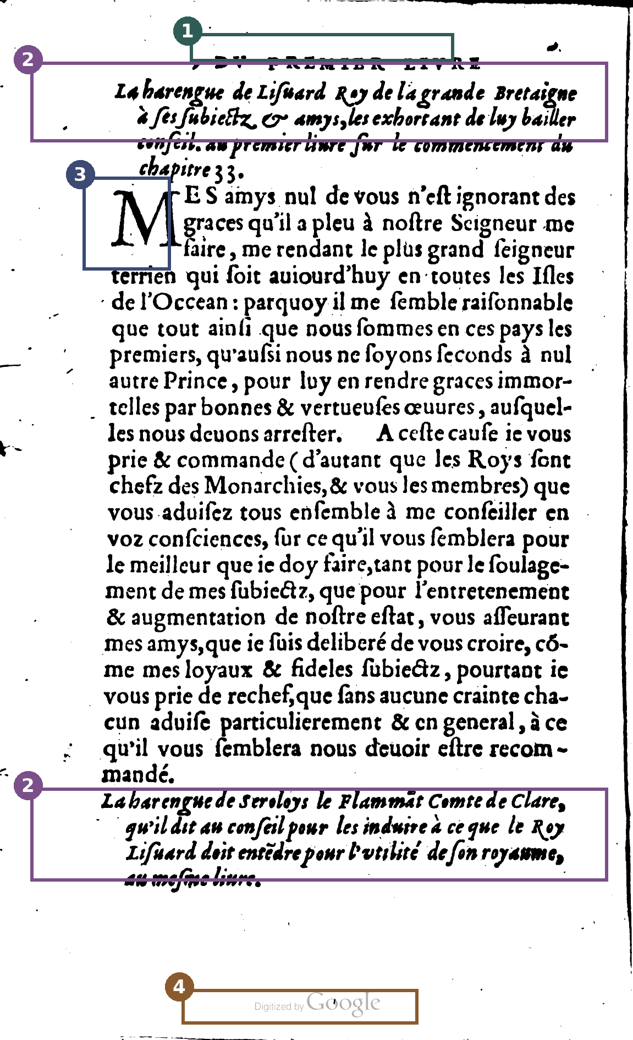
\includegraphics[width=0.62\linewidth]{plates/page-thresor.png}
  \caption{A page of \emph{Le Thresor des douze livres d'Amadis de Gaule}
    (1559), an earlier edition of the \emph{Trésor} than the 1582 one the model
    was fine-tuned on. \textbf{1} running head,
    \qtr{DV PREMIER LIVRE}. \textbf{2} italic rubrics, which the layout stage
    turns into titles because of their slant. \textbf{3} the drop cap \qtr{M}
    of \qtr{MES amys}, which line segmentation misses. \textbf{4} the
    digitiser's watermark, caught as a possible footer and left out of the
    text. Long \qtr{ſ} throughout. The numbered overlay was added for this
    figure.}
  \label{fig:plate}
\end{figure}

\subsection{Two editions}

The \ocrBooks{} books are not one edition. The first \ocrBooksFamilyA{}
(family~A, \ocrPagesFamilyA{} pages) are a large folio edition in
\emph{bâtarde} type, with roman folio numbers and a printed table of contents
in each volume. The other \ocrBooksFamilyB{} (family~B, \ocrPagesFamilyB{}
pages) are later and smaller, in roman type with italic rubrics, arabic page
numbers and no table of contents. Correction results are given per family.
Chapter detection can only be checked on family~A, since it needs a printed
table of contents to compare against.

\subsection{The \emph{Trésor} extracts and the training pages}

The reference for passage location is the editor's catalogue, released as a
CSV file (appendix~\ref{app:data}). For each of its \corpusPieces{} extracts,
the editor noted the Livre it comes from and, where possible, the chapter. For
\corpusCertain{} extracts (\corpusCertainShare{}) the editor is sure. For the
others the editor is unsure, marking \corpusUncertain{} with a question mark and
giving \corpusConjecture{} as a guess in brackets, or gives no location at all
(\corpusUnassigned{}). The locator is scored only on the extracts whose
location is sure, since the others have no reliable answer to check against.
The
locator placed \corpusAligned{} extracts across \corpusLivres{} of the
\ocrBooks{} books. The median extract is \corpusCharsMedian{} characters long,
the longest \corpusCharsMax{}.

The recogniser was trained on \trainPages{} pages transcribed in Transkribus,
all from \emph{Trésor des Amadis}~T.1: \trainPagesTrain{} for training and
\trainPagesVal{} held out for validation. No page of \emph{Amadis de Gaule} was
added to the training set. Its pages are much easier to read than those of the
\emph{Trésor}, and the base CATMuS-Print model already read them well without
fine-tuning, so the training effort went to the harder volume.

\subsection{The pipeline}
\label{sec:system}

\begin{figure}[t]
  \centering
  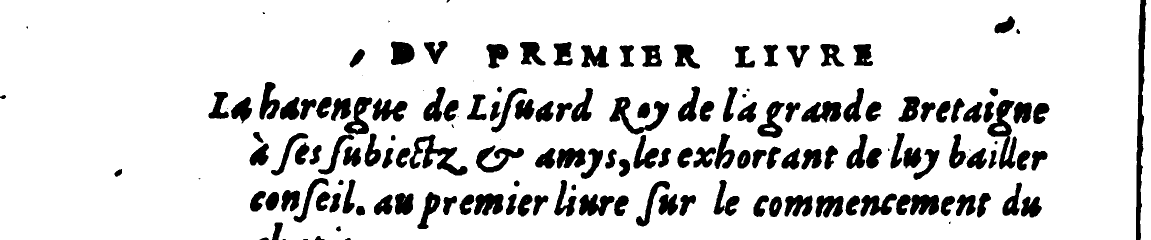
\includegraphics[width=0.86\linewidth]{plates/spec-rubric.png}\\[0.35em]
  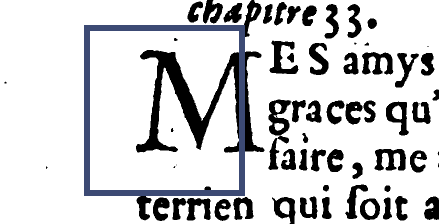
\includegraphics[width=0.33\linewidth]{plates/spec-dropcap.png}\hfill
  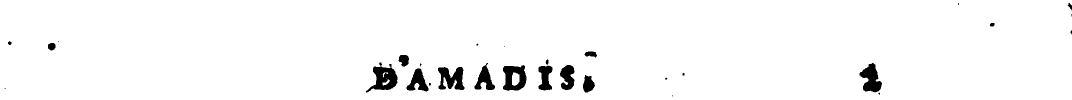
\includegraphics[width=0.60\linewidth]{plates/spec-header.png}
  \caption{What the layout stage looks at: geometry only. Top: body text sits
    near $0^\circ$ while this rubric slants 12--18$^\circ$ against the page's
    median, so slant marks a title and the wording never does. Bottom left: an
    ink blob 1.6--9 times the line height, with an aspect ratio of 0.4--1.8, in
    the left 20\% of the column is a drop cap. Bottom right: a short centred
    line with a folio number is a running head.}
  \label{fig:layout}
\end{figure}

\textbf{Recognition} uses kraken~7.0.2 \cite{kiessling2025kraken} with a model
fine-tuned from CATMuS-Print [Large] \cite{gabay2024catmusprintlarge} on the
training pages above. I ran two configurations. The first kept kraken's default
constant learning rate of $10^{-3}$. The second, which is the one shipped,
started at $3\times10^{-4}$, halved the rate whenever validation stopped
improving, and added data augmentation. The shipped model file is tied to its
training checkpoint by comparing weights, and its hash is recorded in the
repository (appendix~\ref{app:data}).

\textbf{Layout} uses no learned model (figure~\ref{fig:layout}). Baselines give
the reading order, oversized or slanted lines become titles, lines in the top
and bottom margins become headers and footers, and illustrations and library
stamps are left out. Geometry cannot decide the case of a single line at the
top or bottom of a page, which may be a running head, a catchword, or the first
or last line of the text. A first language-model pass handles these lines by
checking whether their neighbours read on naturally once the line is removed.

\textbf{Correction} marks every word that contains a character scored below a
confidence threshold, by wrapping it in \lmark~\rmark{}, and sends the
line to a local language model with the two lines around it for context. The
prompt forbids modernising the spelling. The reply is split on the markers and
kept only if it has the same number of markers and every character outside
them is identical to the original. Otherwise the whole line is left as it was.
A rewrite of the surrounding text is therefore easy to detect and refuse,
however plausible it looks. Both language-model passes are optional, and both
leave the text unchanged when the model is missing or fails.

\textbf{Passage location} searches the full transcription of all \ocrBooks{}
books. A normaliser first folds the spelling variation of the period. Rare
words, with a minimum length and a maximum number of occurrences, act as seeds that propose candidate positions.
The candidates are chained into a span within each book, and the best span is
accepted if its score is above an accept threshold. The locator returns that
span and the Livre it falls in. A chapter can then be read from the chapter
heading above the span, as the pipeline transcribed it.

The pipeline's behaviour depends on a handful of settings:
\begin{itemize}
  \item the \textbf{correction confidence threshold}: a word containing a
    character scored below it counts as doubtful and is sent for correction;
  \item the \textbf{drop-cap probability threshold}: a small image model names
    the letter of each drop cap, and when its confidence falls below this value
    a larger model is asked instead;
  \item the \textbf{minimum seed length} and \textbf{maximum seed occurrences}:
    they decide which words are rare enough to serve as seeds, since short or
    frequent words point to too many places;
  \item the \textbf{chaining gap penalty}: the cost of a gap between two seeds,
    kept low enough that an extract with a cut in it still chains across the
    cut;
  \item the \textbf{chaining window margin}: how much text either side of a
    chain is taken before the span's limits are fixed;
  \item the \textbf{location accept threshold}: the minimum score for a span to
    be accepted as the extract's location.
\end{itemize}
Only the location accept threshold is checked in this report
(section~\ref{sec:e5}). Appendix~\ref{app:data} gives each setting's name in
the code.
